\section{Algebraic Expressions}
A \textbf{variable} is a letter that can represent any number from a given set of numbers. If we
start with variables, such as $x$, $y$, and $z$, and some real numbers and combine them using
addition, subtraction, multiplication, division, powers, and roots, we obtain an \textbf{algebraic expression}. Here are some examples:

$$ 
    2x^2-3x+4 \quad \sqrt{x}+10 \quad \frac{y-2z}{y^2+4}
$$

A \textbf{monomial} is an expression of the form $ax^k$
, where a is a real number and k is a
nonnegative integer. A \textbf{binomial} is a sum of two monomials and a \textbf{trinomial} is a sum
of three monomials. In general, a sum of monomials is called a \textbf{polynomial}. For example, the first expression listed above is a polynomial, but the other two are not.

\begin{align*}
    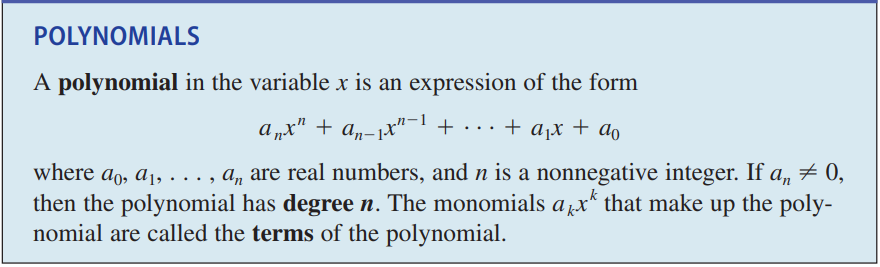
\includegraphics[width=1.1\textwidth]{algebra-pre-calculus/algebra/algebraic-expressions/polynomial definition.png}
\end{align*} \break

Note that the degree of a polynomial is the highest power of the variable that appears
in the polynomial.


\begin{align*}
    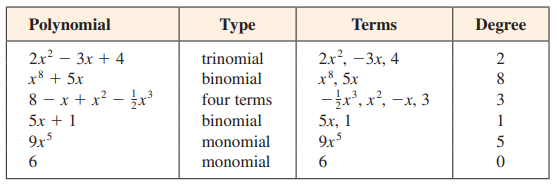
\includegraphics[width=1.1\textwidth]{algebra-pre-calculus/algebra/algebraic-expressions/algebraic-expression-spreadsheet.png}
\end{align*} \break

We add and subtract polynomials using the properties of real numbers that were discussed earlier. The idea is to combine like terms (that is, terms with the same
variables raised to the same powers) using the Distributive Property. For instance,

$$ 
    5x^7+3x^7-2x^7 = (5+3-2)x^7 = 6x^7
$$

But we already know this. 

To find the product of polynomials or other algebraic expressions, we need to use the
Distributive Property repeatedly. In particular, using it three times on the product of two
binomials, we get

$$ 
    (a+b)(c+d) = a(c+d)+b(c+d) = ac+ad+bc+bd
$$

\subsection{Special Product Formulas}
Certain types of products occur so frequently that you should memorize them. You can
verify the following formulas by performing the multiplications.

\begin{align*}
    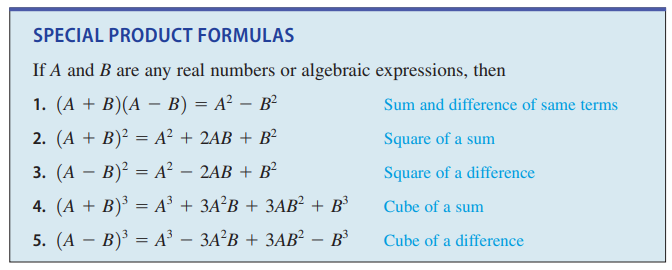
\includegraphics[width=1.1\textwidth]{algebra-pre-calculus/algebra/algebraic-expressions/special_product_formulas.png}
\end{align*} \break

\subsection{Factoring Common Factors}
We use the Distributive Property to expand algebraic expressions. We sometimes need
to reverse this process (again using the Distributive Property) by factoring an expression as a product of simpler ones.
For example,
\begin{align*}
    &A. \quad 15 + 25x = 5(3 + 5x) \\
    &B. \quad x^2y + y^2x^3 = x^2y(1 + xy) \\
\end{align*}
You can always check whether you have factored correctly by expanding the brackets.

\subsection{Factoring quadratics}
A quadratic is an expression with a squared term, then just a term with a variable, then a constant. 
\\ Like this: $ax^2 + bx + c$ 
More about solving quadratic equations and quadratic equations in general can be found in the next section \hyperref[sec:quadratic-equations]{Quadratic Equations(click to redirect)}.


We are looking for two numbers that multiply you get $c$ and when you add them you get $b$.
The reason why: 
$$ (x + m)(x + n) = \\ x^2 + mx + nx + mn = x^2 + \underbrace{(m + n)}_b x + \underbrace{(mn)}_c $$

$m$ and $n$ are the two numbers we are looking for. As you can see $m + n = b$ and $mn = c$. \\

\textbf{Example}. Factor $x^2 - 6x + 8$ \\
We are looking for two numbers that multiply you get $8$ and when you add them you get $-6$. \\
The two numbers are $-2$ and $-4$ because $-2 \cdot -4 = 8$ and $-2 + -4 = -6$. \\
Therefore, 
\begin{align*}
    x^2 - 6x + 8 &= (x - 2)(x - 4) \\
\end{align*}

\textbf{Example}. Factor $10x^2 + 11x - 6$ \\
\begin{itemize}
    \item Step 1. Multiply the leading coefficient (10) and the constant term (-6) to get -60. \\
    \textbf{Why?} The main goal in factoring a quadratic equation is to express it as the product of two binomials(like (2x+4)(4x+5)). 
    In the case of a quadratic with a leading coefficient (the coefficient of $x^2$) not equal to 1, like $10x^2$ in our example, we need to find two binomials of the form $(ax + b)(cx + d)$ e.g $(2x + 4)(5x+2)$ such that their product equals the given quadratic. 
    So, in this context, we are essentially trying to break down the original quadratic ($10x^2 - 11x - 6$) into two binomials, and we start by looking for two numbers that will help us achieve this. These two numbers should meet two criteria:
    \begin{itemize}
        \item Their product should equal the product of the leading coefficient and the constant term (in this case, $10 \cdot -6 = -60$).
        \item Their sum should equal the coefficient of the x-term (in this case, -11)
    \end{itemize}
    By finding such numbers, we can rewrite the middle term of the quadratic equation (the -11x term) as the sum or difference of two terms, each of which can be factored more easily. This allows us to perform factoring by grouping, making the overall factoring process more manageable.
    \item Step 2.  Find two numbers that multiply to -60 and add up to the coefficient of the x-term (-11). In this case, those two numbers are -15 and 4 because $(-15) \cdot 4 = -60$ and $(-15) + 4 = -11$.
    \item Step 3. Rewrite the middle term (-11x) using the two numbers found in step 2: 
    $$ 10x^2 - 15x + 4x - 6 $$
    \item Step 4. Group the terms: Group the first two terms $(10x^2 - 15x)$ and the last two terms $(4x - 6)$. This will gve us: 
    $$ 5x(2x - 3) + 2(2x - 3) $$
    \item Step 5. Factor out the HCF of each group: 
    $$ 5x(2x - 3) + 2(2x - 3) = (5x + 2)(2x - 3) $$

\end{itemize}
And we are done factorising the quadratic equation.

\subsection{Difference of squares}
The difference of squares is a squared term minus another squared term.
\\ Like this: $a^2 - b^2 = (a+b)(a-b) = a^2-ab+ab-b^2 $ 

\textbf{Example.} Factor $x^2 - 9$ 
$$ (x+3)(x-3) $$


\textbf{Example.} Factor $9p^2 - 1$ 
$$ (3p+1)(3p-1) $$

\subsection{Difference or sum of cubes}
The difference or sum of cubes is a cubed term plus or minus another cubed term.

$$ a^3 - b^3 = (a-b)(a^2+ab+b^2) $$ Because, $$(a-b)(a^2+ab+b^2) = a^3 - ab^2 + a^2b - ab^2 + b^3 = a^3 - 2ab^2 + b^3 $$ 

And, 
$$ a^3 + b^3 = (a+b)(a^2-ab+b^2) $$ Because, $$(a+b)(a^2-ab+b^2) = a^3 + ab^2 - a^2b + ab^2 + b^3 = a^3 + 2ab^2 + b^3 $$ 
\\
\textbf{Example.} Factor $x^3 - 8$ \\
We know that $x^3 - 8 = x^3 - 2^3$
Therefore,
$$ (x-2)(x^2+2x+4) $$

if we expand out: 
$$ (x-2)(x^2+2x+4) = x^3 + 2x^2 + 4x - 2x^2 - 4x - 8 = x^3 - 8 $$
Therefore our answer is correct.

\subsection{Additional examples of factoring}
\textbf{Example.} Which of these expressions DOES NOT factorise?

A. $x^2 + x$ \\
This can be factored by pulling out the highest common factor. \\
$$ x^2 + x = x(x+1) $$

B. $x^2 - 25$ \\
This also can be factored by difference of squares. \\
$$ x^2 - 25 = (x+5)(x-5) $$

C. $x^2 + 4$ \\
This cannot be factored because it is a sum of squares not a difference of squares. \\

D. $x^3+2x^2+3x+6$ \\
This can also be factored by grouping. \\
$$ x^3+2x^2+3x+6 = x^2(x+2)+3(x+2) = (x^2+3)(x+2) $$

E. $5x^2-14x+8$ \\
This can also be factored by using the method of factoring quadratics when $a \neq 1$. \\
Therefore we can multiply the leading coefficient (5) and the constant term (8) to get 40. \\
We are looking for two numbers that multiply you get 40 and when you add them you get -14 and those are -10 and -4. \\
So we can rewrite the middle term (-14x) using the two numbers found:
$$ 5x^2 - 10x - 4x + 8 $$ 
Then we can group them together:
$$ 5x(x - 2) - 4(x - 2) $$
And finally factor out the HCF of each group:
$$ (5x - 4)(x - 2) $$

Eventually the answer for our question is C. $x^2 + 4$ because it cannot be factored.

\subsection{Tips and Extra examples}
\begin{itemize}
    \item Always look for the highest common factor first. That will simplify things and make the rest of the factoring more easier. 
    \item You might need to do several steps of factoring to get the final answer. For example you might have to pull out the HCF first then you can do factoring by grouping or factoring quadratics. Then you might also apply difference of squares or difference or sum of cubes. Keep factoring as far as you can go.
\end{itemize}

\textbf{Extra Example} Factor $2z^2 + 3z -14$ \\
Again as previously done first we need to multiply the leading coefficient (2) and the constant term (-14) to get -28. \\ 
We are looking for two numbers that multiply you get -28 and when you add them you get 3 and those are 7 and -4. \\
So we can rewrite the middle term (3z) using the two numbers found:
$$ 2z^2 + 7z - 4z - 14 $$ 
Then we can group them together:
$$ z(2z + 7) - 2(2z + 7) $$
And finally factor out the HCF of each group:
$$ (z - 2)(2z + 7) $$

\textbf{Extra Example} Factor $-5v^2-45v+50$ \\
Again as previously done first we need to multiply the leading coefficient (-5) and the constant term (50) to get -250. \\
We are looking for two numbers that multiply you get -250 and when you add them you get -45 and those are -50 and 5. \\
So we can rewrite the middle term (-45v) using the two numbers found:
$$ -5v^2 - 50v + 5v + 50 $$ 
Then we can group them together:
$$ -5v(v + 10) + 5(v + 10) $$
And finally factor out the HCF of each group:
$$ (-5v + 5)(v + 10) $$
This can be further simplified to:
$$ -5(v - 1)(v + 10) $$
Another solution for this could have been that first we could have pulled out the HCF which is -5 and then we could have factored the quadratic. \\
$$ -5v^2 - 45v + 50 = -5(v^2 + 9v - 10) $$
And this is really easy since $ a = 1 $ Therefore we need two numbers that multiply you get -10 and when you add them you get 9 and those are 10 and -1. \\
So we can say that: 
$$ -5(v^2 + 9v - 10) = -5(v + 10)(v - 1) $$

\subsection{Special Factoring Formulas}
\begin{align*}
    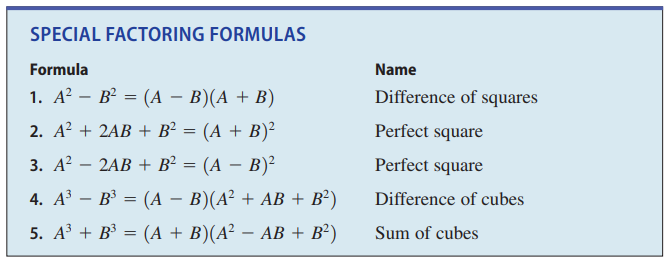
\includegraphics[width=1.1\textwidth]{algebra-pre-calculus/algebra/algebraic-expressions/special_factoring_formulas.png}
\end{align*} \break

When we factor an expression, the result can sometimes be factored further. In general, we first factor out common factors, then inspect the result to see whether it can be
factored by any of the other methods of this section. We repeat this process until we
have factored the expression completely

\subsection{Factoring Expressions with Fractional Exponents}
Factor each expresson. \\ \break
\textbf{(a)} \scalebox{1.2}{$3x^{\frac{3}{2}}-9x^{\frac{1}{2}}+6x^{-\frac{1}{2}}$ = $3x^{-\frac{1}{2}}(x^2-3x+2)$ = $3x^{-\frac{1}{2}}(x-2)(x-1)$} \\ \break
Here we have taken the common factor $3x^{-\frac{1}{2}}$ out of each term. Then we have factored the quadratic expression $x^2-3x+2$. \\ \break

\textbf{(b)} $(2+x)^{-\frac{2}{3}}x+(2+x)^{\frac{1}{3}} = (2+x)^{-\frac{2}{3}}[x+(2+x)] = (2+x)^{-\frac{2}{3}}(x+2+x) = (2+x)^{-\frac{2}{3}}(2x+2)$ \\ \break
Here we have taken the common factor $(2+x)^{-\frac{2}{3}}$ out of each term. Then we have just simplified. \\ \break